\documentclass[aspectratio=169, 10pt, professionalfonts]{beamer}

% ==============================================================================
% PRESENTATION THEME & COLOR CONFIGURATION
% ==============================================================================
\usetheme{Madrid}
\useinnertheme{rectangles}
\usefonttheme{structurebold}

% Professional Academic Color Palette (Deep Navy, Slate Blue, Teal Accent)
\definecolor{NavyDark}{RGB}{15, 34, 64}
\definecolor{NavyBlue}{RGB}{27, 59, 111}
\definecolor{SlateGray}{RGB}{80, 90, 105}
\definecolor{TealAccent}{RGB}{0, 128, 128}
\definecolor{LightGrayBg}{RGB}{246, 248, 250}
\definecolor{BorderGray}{RGB}{210, 215, 222}
\definecolor{AlertRed}{RGB}{185, 28, 28}
\definecolor{SafeGreen}{RGB}{22, 101, 52}
\definecolor{WarningAmber}{RGB}{180, 83, 9}

\setbeamercolor{palette primary}{bg=NavyDark, fg=white}
\setbeamercolor{palette secondary}{bg=NavyBlue, fg=white}
\setbeamercolor{palette tertiary}{bg=SlateGray, fg=white}
\setbeamercolor{structure}{fg=NavyBlue}
\setbeamercolor{frametitle}{bg=NavyDark, fg=white}
\setbeamercolor{title}{bg=NavyDark, fg=white}
\setbeamercolor{author}{fg=white}
\setbeamercolor{date}{fg=white!85}
\setbeamercolor{institute}{fg=white!85}
\setbeamercolor{block title}{bg=NavyBlue, fg=white}
\setbeamercolor{block body}{bg=LightGrayBg, fg=black}
\setbeamercolor{block title example}{bg=TealAccent, fg=white}
\setbeamercolor{block body example}{bg=LightGrayBg, fg=black}
\setbeamercolor{block title alerted}{bg=AlertRed, fg=white}
\setbeamercolor{block body alerted}{bg=LightGrayBg, fg=black}

\setbeamertemplate{navigation symbols}{}
\setbeamertemplate{footline}{
  \leavevmode%
  \hbox{%
    \begin{beamercolorbox}[wd=.30\paperwidth,ht=2.25ex,dp=1ex,left,leftskip=1ex]{palette secondary}%
      \textbf{FloodSense} -- 22AIE498 Phase 1
    \end{beamercolorbox}%
    \begin{beamercolorbox}[wd=.45\paperwidth,ht=2.25ex,dp=1ex,center]{palette primary}%
      Multi-Model Framework with RAG-LLM for Flood Reporting
    \end{beamercolorbox}%
    \begin{beamercolorbox}[wd=.25\paperwidth,ht=2.25ex,dp=1ex,right,rightskip=1ex]{palette tertiary}%
      \insertframenumber{} / \inserttotalframenumber
    \end{beamercolorbox}%
  }%
  \vskip0pt%
}

% ==============================================================================
% REQUIRED PACKAGES
% ==============================================================================
\usepackage[utf8]{inputenc}
\usepackage{lmodern}
\usepackage{amsmath, amssymb, mathtools}
\usepackage{booktabs}
\usepackage{tabularx}
\usepackage{array}
\usepackage{multirow}
\usepackage{tikz}
\usetikzlibrary{shapes.geometric, arrows.meta, positioning, calc, fit, backgrounds, shadows}
\usepackage{hyperref}
\hypersetup{
    colorlinks=true,
    linkcolor=NavyBlue,
    urlcolor=TealAccent,
    citecolor=NavyBlue
}

% Custom table column types
\newcolumntype{Y}{>{\raggedright\arraybackslash}X}
\newcolumntype{C}{>{\centering\arraybackslash}X}
\newcolumntype{m}{>{\raggedright\arraybackslash}p}

% ==============================================================================
% TITLE & METADATA
% ==============================================================================
\title[FloodSense: Multi-Model Flood Reporting]{\textbf{FloodSense: A Multi-Model Framework with RAG-LLM System for Automated Flood Reporting}}
\subtitle{\large 22AIE498 Project Phase 1}
\author[Group C-06]{%
  \textbf{Group C-06}\\[0.6em]
  Varshitha Thilak Kumar \quad (CB.SC.U4AIE23258)\\[0.2em]
  Siri Sanjana S \quad (CB.SC.U4AIE23249)\\[0.2em]
  Shreya Arun \quad (CB.SC.U4AIE23253)\\[0.2em]
  Anagha Menon \quad (CB.SC.U4AIE23212)
}
\institute[Amrita Vishwa Vidyapeetham]{
  Department of Artificial Intelligence\\
  School of Computing, Amrita Vishwa Vidyapeetham\\[0.5em]
  \textbf{Project Supervisor:} Dr.~Mithun Kumar Kar
}
\date{October 2026}

\begin{document}

% ==============================================================================
% SLIDE 1: TITLE SLIDE
% ==============================================================================
\begin{frame}[plain]
  \titlepage
\end{frame}

% ==============================================================================
% SLIDE 2: INTRODUCTION & MOTIVATION
% ==============================================================================
\begin{frame}{Introduction \& Motivation}
  \begin{columns}[T]
    \begin{column}{0.5\textwidth}
      \begin{block}{The Disaster Challenge}
        \begin{itemize}\setlength{\itemsep}{0.6em}
          \item \textbf{High-Impact Calamity:} Floods represent one of the most destructive natural disasters, causing catastrophic loss of life, infrastructure failure, and displacement.
          \item \textbf{The Golden Hour Bottleneck:} Manual ground inspection cannot scale during rapid-onset, large-scale inundations. Rapid and precise assessment is essential for efficient triage.
          \item \textbf{Operational Blindspots:} Responders need immediate, reliable situational awareness, but field access is frequently severed by inundated road networks.
        \end{itemize}
      \end{block}
    \end{column}
    
    \begin{column}{0.5\textwidth}
      \begin{block}{Current Technological Gap}
        \begin{itemize}\setlength{\itemsep}{0.6em}
          \item \textbf{Detection vs. Actionable Intelligence:} Existing AI approaches either generate binary water masks without contextual impact, or produce ungrounded textual reports lacking visual verification.
          \item \textbf{Risk of Hallucination:} Pure LLM-based disaster synthesizers hallucinate critical damage statistics in the absence of rigorous spatial anchoring.
          \item \textbf{The FloodSense Solution:} Seamlessly bridges multi-model Computer Vision (CV) with Statutory Retrieval-Augmented Generation (RAG) to generate legally traceable, evidence-grounded Situation Reports (SITREPs).
        \end{itemize}
      \end{block}
    \end{column}
  \end{columns}
\end{frame}

% ==============================================================================
% SLIDE 3: LITERATURE REVIEW (PAPERS 1 & 2)
% ==============================================================================
\begin{frame}{Literature Review (1/4)}
  \begin{table}[h]
    \scriptsize
    \centering
    \begin{tabularx}{\textwidth}{p{0.4cm} p{3.2cm} Y Y p{2.4cm}}
      \toprule
      \textbf{\#} & \textbf{Title \& Authors} & \textbf{Methodology} & \textbf{Drawbacks} & \textbf{Dataset} \\
      \midrule
      1 & 
      \textbf{DisasTeller: Integration of LVLMs for Post-Disaster Damage Assessment} \newline \textit{Chen et al. (2026)} & 
      Multi-agent LVLM framework integrating RAG with 4 specialised AI agents to automate assessment, alarm generation, and resource planning. & 
      Errors in early damage assessment propagate down the multi-agent pipeline, producing skewed alarms and erroneous resource allocation. & 
      Wajima City earthquake post-disaster imagery case study (Japan). \\
      \midrule
      2 & 
      \textbf{Explainable Flood Damage Assessment via MASA \& VLM} \newline \textit{Aydin et al. (2026)} & 
      Couples LoRA-fine-tuned BLIP-2 VLM with MASA-enhanced DeepLabV3+ for multi-scale flood segmentation and report captioning. & 
      Two independently trained models; segmentation mask is not mathematically passed into the VLM prompt, preventing end-to-end reasoning. & 
      FloodNet (UAV orthophotos) and LADI-v2 (10k low-altitude aerial images). \\
      \bottomrule
    \end{tabularx}
  \end{table}
\end{frame}

% ==============================================================================
% SLIDE 4: LITERATURE REVIEW (PAPERS 3 & 4)
% ==============================================================================
\begin{frame}{Literature Review (2/4)}
  \begin{table}[h]
    \scriptsize
    \centering
    \begin{tabularx}{\textwidth}{p{0.4cm} p{3.2cm} Y Y p{2.4cm}}
      \toprule
      \textbf{\#} & \textbf{Title \& Authors} & \textbf{Methodology} & \textbf{Drawbacks} & \textbf{Dataset} \\
      \midrule
      3 & 
      \textbf{CrisiSense-RAG: Crisis Sensing Multimodal RAG} \newline \textit{Xiao et al. (2026)} & 
      Split-pipeline architecture with separate Text and Visual Analyst modules connected by a temporal-aware fusion engine. & 
      Evaluated strictly on Hurricane Harvey; highly sensitive to noise, temporal latency, and sparsity in social media text streams. & 
      NOAA high-resolution aerial tiles, filtered emergency tweets, 911 calls, and rainfall sensors. \\
      \midrule
      4 & 
      \textbf{Training-Free RAG with Reinforced Reasoning for Nowcasting} \newline \textit{Huang et al. (2026)} & 
      3-level reasoning knowledge base with local neighbour retrieval, HUC12 prototypes, reinforced reasoning, and rule-based downgrading. & 
      Dependent on pre-existing historical tabular insurance records; cannot generalize to unmapped or developing geographies lacking NFIP data. & 
      15,378 labeled 500m$\times$500m grid cells in Harris County, Texas (NFIP + FEMA IA claims). \\
      \bottomrule
    \end{tabularx}
  \end{table}
\end{frame}

% ==============================================================================
% SLIDE 5: LITERATURE REVIEW (PAPERS 5 & 6)
% ==============================================================================
\begin{frame}{Literature Review (3/4)}
  \begin{table}[h]
    \scriptsize
    \centering
    \begin{tabularx}{\textwidth}{p{0.4cm} p{3.2cm} Y Y p{2.4cm}}
      \toprule
      \textbf{\#} & \textbf{Title \& Authors} & \textbf{Methodology} & \textbf{Drawbacks} & \textbf{Dataset} \\
      \midrule
      5 & 
      \textbf{Remote Sensing RAG: Bridging RS Imagery \& Knowledge} \newline \textit{Wen et al. (2026)} & 
      RSWK and RS-RAG framework encoding text and imagery in shared vector space; cross-modal retrieval fused into VLM prompts for VQA. & 
      Heavy computational latency during cross-modal retrieval; fixed landmark knowledge base lacks disaster response protocol adaptability. & 
      RSWK benchmark: 14,820 high-resolution satellite landmark images across 184 countries. \\
      \midrule
      6 & 
      \textbf{Multimodal Mamba for Building Damage Assessment} \newline \textit{Ho \& Mostafavi (2025)} & 
      Semi-Siamese Mamba state-space encoder fusing SAR/InSAR with VHR optical basemaps and flood-risk layers via multi-task decoders. & 
      Ground-truth claims under-represent uninsured civilian structures; severe radar speckle degrades fine-scale urban vehicle identification. & 
      UrbanSARFloods (Sentinel-1 SAR from 18 global floods) paired with pre-event optical footprints. \\
      \bottomrule
    \end{tabularx}
  \end{table}
\end{frame}

% ==============================================================================
% SLIDE 6: LITERATURE REVIEW (PAPERS 7 & 8)
% ==============================================================================
\begin{frame}{Literature Review (4/4)}
  \begin{table}[h]
    \scriptsize
    \centering
    \begin{tabularx}{\textwidth}{p{0.4cm} p{3.2cm} Y Y p{2.4cm}}
      \toprule
      \textbf{\#} & \textbf{Title \& Authors} & \textbf{Methodology} & \textbf{Drawbacks} & \textbf{Dataset} \\
      \midrule
      7 & 
      \textbf{LLMArk: Instance-Aware Foundation Model for Flood Risk} \newline \textit{Wu et al. (2026)} & 
      Instance-aware MLLM integrating LoRA-fine-tuned vision-language backbone with a YOLO-based Instance Perception Token. & 
      Proprietary annotations restrict public reproducibility; heavily susceptible to occluded or partially submerged micro-instances. & 
      VLFRA dataset: 50k flood QA pairs, 12k annotated human/vehicle instances, 5k real-world photos. \\
      \midrule
      8 & 
      \textbf{DisasterM3: Vision-Language Dataset for Damage Assessment} \newline \textit{Wang et al. (2026)} & 
      Multi-hazard, multi-sensor benchmark spanning 9 disaster tasks with 123k instruction pairs for VLM evaluation. & 
      Serves as an evaluation benchmark rather than an integrated end-to-end operational SITREP generation system. & 
      DisasterM3: 26,988 bi-temporal optical/SAR image pairs across 36 historical global events. \\
      \bottomrule
    \end{tabularx}
  \end{table}
\end{frame}

% ==============================================================================
% SLIDE 7: RESEARCH GAP
% ==============================================================================
\begin{frame}{Research Gap}
  \begin{block}{Critical Structural Deficiencies in Existing Systems}
    \begin{itemize}\setlength{\itemsep}{0.7em}
      \item \textbf{The Visual-Semantic Decoupling:} Current systems either output an isolated semantic mask (leaving severity scoring, cut-off asset calculations, and logistics drafting to exhausted human responders) or produce purely generative text from secondary web scraping.
      \item \textbf{Absence of Traceable Grounding:} No extant pipeline directly couples fine-grained, 10-class pixel segmentations with LLM synthesis such that \textit{every metric claim in the report is mathematically verifiable against pixel evidence}.
      \item \textbf{Vulnerability in the Early Golden Hour:} Secondary-source text systems fail completely when internet and telecommunication nodes collapse during a disaster, as authoritative web coverage is unavailable.
      \item \textbf{Lack of Statutory Rigor:} Generic LLMs hallucinate evacuation procedures and boat deployment ratios; emergency managers require deterministic compliance with statutory authorities (NDMA, NDRF, FEMA).
    \end{itemize}
  \end{block}
\end{frame}

% ==============================================================================
% SLIDE 8: PROBLEM STATEMENT, SCOPE & BOUNDARIES
% ==============================================================================
\begin{frame}{Problem Statement, Scope \& Boundaries}
  \begin{exampleblock}{Problem Statement}
    \small
    ``Current flood assessment systems are inadequate in two ways: text-based systems generate reports from secondary web sources without direct visual grounding, making them slow, incomplete, and unverifiable against actual site imagery; segmentation-only models identify flooded regions but leave severity interpretation and reporting to humans. At the moment, no solution combines report production with fine-grained flood segmentation so that each claim may be linked to visual proof.''
  \end{exampleblock}

  \vspace{0.4em}
  \begin{columns}[T]
    \begin{column}{0.5\textwidth}
      \begin{block}{System Scope}
        \begin{itemize}\footnotesize
          \item End-to-end demo dashboard for rapid aerial flood triage.
          \item 5-paradigm Computer Vision benchmark (HSV to SegFormer).
          \item Pixel-calibrated spatial metrics ($A_{\text{water}}$, $R_{\text{bld}}$, $R_{\text{road}}$, $N_{\text{veh}}$).
          \item ChromaDB RAG indexing NDMA/FEMA statutory protocols.
          \item Automated multi-format SITREP generation (PDF, DOCX, JSON).
        \end{itemize}
      \end{block}
    \end{column}
    
    \begin{column}{0.5\textwidth}
      \begin{block}{Project Boundaries}
        \begin{itemize}\footnotesize
          \item Focuses on post-event UAV aerial orthophotos and calibrated bench datasets.
          \item Knowledge base bounded by authoritative statutory guidelines (NDMA, NDRF, FEMA).
          \item Real-time drone stream ingestion is modeled via calibrated tile ingestion (proof-of-concept scope).
          \item Non-flood disaster categories (wildfires, earthquakes) excluded from primary segmentation decoders.
        \end{itemize}
      \end{block}
    \end{column}
  \end{columns}
\end{frame}

% ==============================================================================
% SLIDE 9: OBJECTIVES
% ==============================================================================
\begin{frame}{Objectives}
  \begin{columns}[T]
    \begin{column}{0.5\textwidth}
      \begin{block}{Computer Vision Objectives}
        \begin{itemize}\setlength{\itemsep}{0.6em}\footnotesize
          \item \textbf{Multi-Class Granularity:} Move beyond binary flood masks to segment 10 critical disaster classes (flooded/intact roads, flooded/intact buildings, vehicles, water, vegetation, terrain) achieving per-class $\text{F1} \ge 0.75$.
          \item \textbf{5-Model Rigorous Benchmark:} Quantitatively benchmark classical thresholding, SAM, Grounding DINO + SAM 2, SegFormer-B3, and Visual LLMs, targeting global $\text{mIoU} > 0.45$ and Pixel Accuracy $> 80\%$.
          \item \textbf{Monocular Topography:} Integrate relative depth estimation to map flood pooling hollows and identify safe highland staging zones.
        \end{itemize}
      \end{block}
    \end{column}
    
    \begin{column}{0.5\textwidth}
      \begin{block}{RAG, Reporting \& Deployment Objectives}
        \begin{itemize}\setlength{\itemsep}{0.6em}\footnotesize
          \item \textbf{Statutory Retrieval Precision:} Construct a RAG pipeline over NDMA, NDRF, and FEMA guidelines achieving $\text{Precision@1} \ge 85\%$ and $\text{Recall@3} = 100\%$.
          \item \textbf{Zero-Hallucination Groundedness:} Guarantee $\ge 90\%$ of factual statements cite segmentation telemetry or retrieved statutory clauses via verifiable tag citations.
          \item \textbf{Lightweight Field Platform:} Deliver a production-grade web dashboard with end-to-end inference-to-report latency $< 60$ seconds (achieved $< 1.8$s locally).
        \end{itemize}
      \end{block}
    \end{column}
  \end{columns}
\end{frame}

% ==============================================================================
% SLIDE 10: METHODOLOGY OVERVIEW
% ==============================================================================
\begin{frame}{System Methodology: Three-Tier Pipeline}
  \begin{center}
    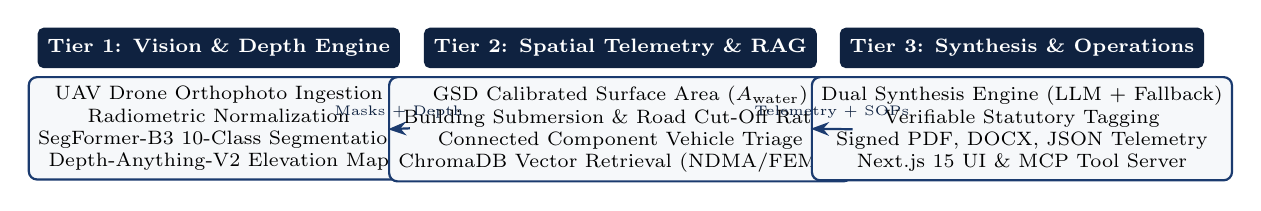
\begin{tikzpicture}[
      box/.style={rectangle, draw=NavyBlue, fill=LightGrayBg, rounded corners=3pt, thick, align=center, font=\scriptsize, minimum height=1.3cm},
      titlebox/.style={rectangle, draw=NavyDark, fill=NavyDark, text=white, font=\bfseries\scriptsize, rounded corners=2pt, minimum height=0.5cm},
      arrow/.style={-{Stealth[scale=1.0]}, thick, NavyBlue}
    ]
      % Tier 1
      \node[titlebox, minimum width=4.3cm] (t1_head) at (0, 2.2) {Tier 1: Vision \& Depth Engine};
      \node[box, minimum width=4.3cm, below=0.1cm of t1_head] (t1_body) {
        UAV Drone Orthophoto Ingestion\\
        Radiometric Normalization\\
        SegFormer-B3 10-Class Segmentation\\
        Depth-Anything-V2 Elevation Map
      };
      
      % Tier 2
      \node[titlebox, minimum width=4.3cm] (t2_head) at (5.1, 2.2) {Tier 2: Spatial Telemetry \& RAG};
      \node[box, minimum width=4.3cm, below=0.1cm of t2_head] (t2_body) {
        GSD Calibrated Surface Area ($A_{\text{water}}$)\\
        Building Submersion \& Road Cut-Off Ratios\\
        Connected Component Vehicle Triage\\
        ChromaDB Vector Retrieval (NDMA/FEMA)
      };
      
      % Tier 3
      \node[titlebox, minimum width=4.3cm] (t3_head) at (10.2, 2.2) {Tier 3: Synthesis \& Operations};
      \node[box, minimum width=4.3cm, below=0.1cm of t3_head] (t3_body) {
        Dual Synthesis Engine (LLM + Fallback)\\
        Verifiable Statutory Tagging\\
        Signed PDF, DOCX, JSON Telemetry\\
        Next.js 15 UI \& MCP Tool Server
      };
      
      % Arrows
      \draw[arrow] (t1_body.east) -- (t2_body.west) node[midway, above, font=\tiny, text=NavyDark] {Masks + Depth};
      \draw[arrow] (t2_body.east) -- (t3_body.west) node[midway, above, font=\tiny, text=NavyDark] {Telemetry + SOPs};
    \end{tikzpicture}
  \end{center}
  \vspace{-0.5em}
  \begin{block}{Key Operational Principle}
    \footnotesize
    Raw pixels are converted into deterministic spatial metrics ($A_{\text{water}}$, $R_{\text{bld}}$, $R_{\text{road}}$, $N_{\text{veh}}$). These metrics trigger targeted semantic queries into the statutory knowledge base, ensuring the LLM acts purely as an evidence-grounded synthesizer rather than an unconstrained generator.
  \end{block}
\end{frame}

% ==============================================================================
% SLIDE 11: DETAILED ARCHITECTURE FLOW DIAGRAM
% ==============================================================================
\begin{frame}{Detailed Architecture Flow Diagram}
  \begin{center}
    \resizebox{0.92\textwidth}{!}{
    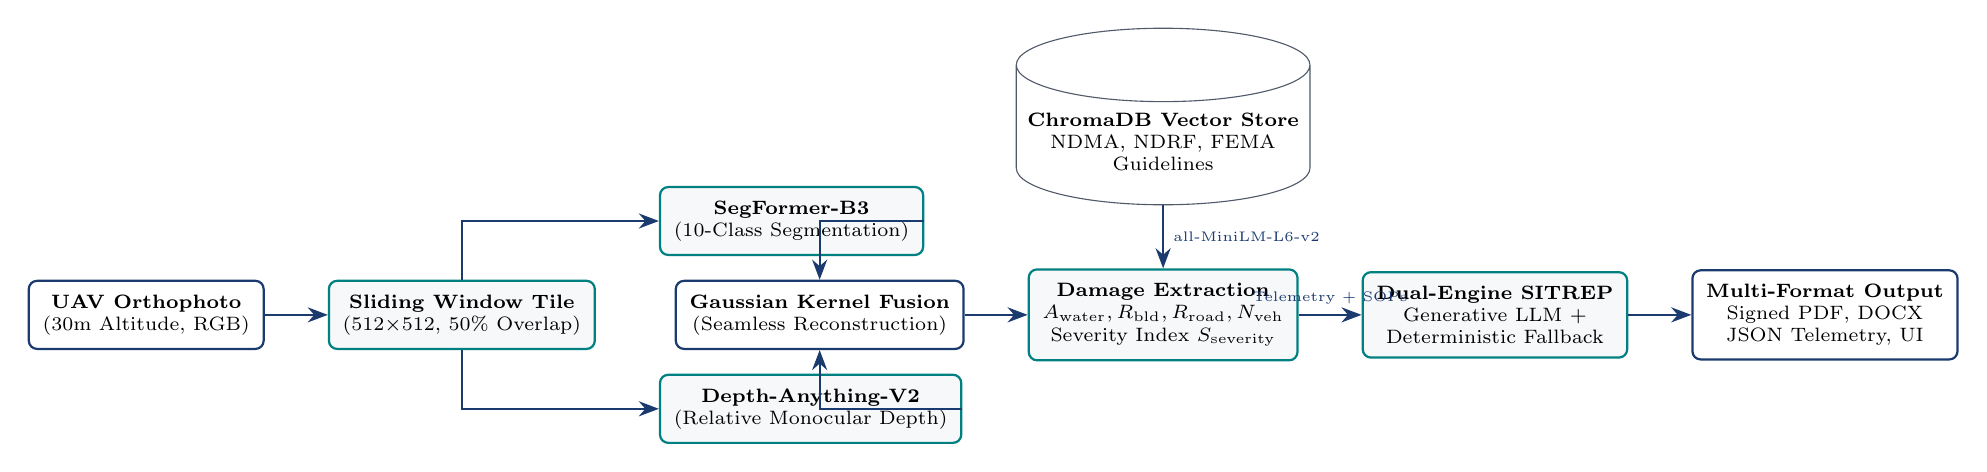
\begin{tikzpicture}[
      node distance=1.4cm and 0.8cm,
      block/.style={rectangle, draw=NavyBlue, fill=white, rounded corners=3pt, thick, align=center, font=\scriptsize, inner sep=5pt},
      proc/.style={rectangle, draw=TealAccent, fill=LightGrayBg, rounded corners=3pt, thick, align=center, font=\scriptsize, inner sep=5pt},
      data/.style={cylinder, draw=SlateGray, fill=white, shape border rotate=90, aspect=0.25, align=center, font=\scriptsize, inner sep=4pt},
      arrow/.style={-{Stealth[scale=1.1]}, thick, NavyBlue}
    ]
      % Nodes
      \node[block] (uav) {\textbf{UAV Orthophoto}\\ (30m Altitude, RGB)};
      \node[proc, right=of uav] (tile) {\textbf{Sliding Window Tile}\\ (512$\times$512, 50\% Overlap)};
      \node[proc, above right=0.3cm and 0.8cm of tile] (seg) {\textbf{SegFormer-B3}\\ (10-Class Segmentation)};
      \node[proc, below right=0.3cm and 0.8cm of tile] (dep) {\textbf{Depth-Anything-V2}\\ (Relative Monocular Depth)};
      \node[block, right=1.0cm of tile] (fuse) {\textbf{Gaussian Kernel Fusion}\\ (Seamless Reconstruction)};
      \node[proc, right=of fuse] (telemetry) {\textbf{Damage Extraction}\\ $A_{\text{water}}, R_{\text{bld}}, R_{\text{road}}, N_{\text{veh}}$\\ Severity Index $S_{\text{severity}}$};
      \node[data, above=0.8cm of telemetry] (kb) {\textbf{ChromaDB Vector Store}\\ NDMA, NDRF, FEMA\\ Guidelines};
      \node[proc, right=of telemetry] (llm) {\textbf{Dual-Engine SITREP}\\ Generative LLM +\\ Deterministic Fallback};
      \node[block, right=of llm] (out) {\textbf{Multi-Format Output}\\ Signed PDF, DOCX\\ JSON Telemetry, UI};

      % Connections
      \draw[arrow] (uav) -- (tile);
      \draw[arrow] (tile) |- (seg);
      \draw[arrow] (tile) |- (dep);
      \draw[arrow] (seg) -| (fuse);
      \draw[arrow] (dep) -| (fuse);
      \draw[arrow] (fuse) -- (telemetry);
      \draw[arrow] (kb) -- (telemetry) node[midway, right, font=\tiny] {all-MiniLM-L6-v2};
      \draw[arrow] (telemetry) -- (llm) node[midway, above, font=\tiny] {Telemetry + SOPs};
      \draw[arrow] (llm) -- (out);
    \end{tikzpicture}
    }
  \end{center}
  \vspace{-0.5em}
  \begin{itemize}\footnotesize
    \item \textbf{Decoupled Sensing \& Reasoning:} Visual processing is isolated from language generation.
    \item \textbf{Guaranteed Determinism:} When API quotas or connectivity fail, the system falls back to strict statutory logic.
  \end{itemize}
\end{frame}

% ==============================================================================
% SLIDE 12: PRIMARY DISASTER BENCHMARK DATASET: FLOODNET
% ==============================================================================
\begin{frame}{Primary Disaster Benchmark Dataset: FloodNet}
  \begin{columns}[T]
    \begin{column}{0.5\textwidth}
      \begin{block}{Dataset Origin \& Sensor Specifications}
        \begin{itemize}\setlength{\itemsep}{0.4em}\footnotesize
          \item \textbf{Disaster Event:} Post-hurricane aerial surveying following Hurricane Harvey (Texas, USA), curated for the IEEE EARS 2021 Challenge.
          \item \textbf{Acquisition Platform:} DJI Mavic Pro UAV quadcopter operating at a standardized nadir flight altitude of $\sim 30\text{ meters}$ (100 ft).
          \item \textbf{Sensor \& Resolution:} 12-Megapixel onboard CMOS camera; native resolution from $4000\times3000$ to $4592\times3072$ pixels.
          \item \textbf{Ground Sampling Distance (GSD):} $\text{GSD} \approx 1.25\text{ cm/pixel}$, enabling exact physical metric conversion ($A = N_{\text{pixels}} \cdot \text{GSD}^2$).
        \end{itemize}
      \end{block}
    \end{column}
    
    \begin{column}{0.5\textwidth}
      \begin{block}{Dataset Splits \& Image Prevalence}
        \begin{table}[h]
          \tiny
          \centering
          \begin{tabularx}{\textwidth}{l C C C}
            \toprule
            \textbf{Metric / Attribute} & \textbf{Train} & \textbf{Validation} & \textbf{Test} \\
            \midrule
            Orthophoto Count & 29 (1,445 tiles) & 450 images & 448 images \\
            Total Masks Evaluated & 1,445 & 450 & 448 \\
            Flood Image Prevalence & 70.5\% & 59.0\% & 65.5\% \\
            Building Image Prevalence & 43.5\% & 56.0\% & 68.5\% \\
            Road Network Prevalence & 61.5\% & 70.0\% & 75.0\% \\
            \textbf{Class Imbalance Ratio} & \textbf{262.4 : 1} & \textbf{206.5 : 1} & \textbf{175.4 : 1} \\
            \bottomrule
          \end{tabularx}
        \end{table}
        \vspace{-0.5em}
        \begin{itemize}\setlength{\itemsep}{0.2em}\tiny
          \item \textbf{Total Benchmark Scale:} 927 high-res orthophotos; 2,343 pixel-level semantic masks.
          \item \textbf{Tiling Pipeline:} Training split sliced into $512\times512$ patches with $50\%$ overlap (1,445 tiles).
        \end{itemize}
      \end{block}
    \end{column}
  \end{columns}
\end{frame}

% ==============================================================================
% SLIDE 13: 10-CLASS SEMANTIC BREAKDOWN & CLASS IMBALANCE
% ==============================================================================
\begin{frame}{10-Class Semantic Breakdown \& Class Imbalance}
  \begin{table}[h]
    \scriptsize
    \centering
    \begin{tabularx}{\textwidth}{c l C C Y}
      \toprule
      \textbf{ID} & \textbf{Semantic Class} & \textbf{Val Pixels (\%)} & \textbf{Test Pixels (\%)} & \textbf{Disaster Tactical Significance} \\
      \midrule
      0 & Background & 0.85\% & 0.93\% & Unlabeled periphery / border padding \\
      1 & Building - Flooded & 2.22\% & 3.69\% & Submerged residential \& commercial structures \\
      2 & Building - Non-Flooded & 3.46\% & 4.72\% & Structurally sound civilian shelters \& staging \\
      3 & Road - Flooded & 3.72\% & 4.99\% & Severed transportation corridors \& cut-off nodes \\
      4 & Road - Non-Flooded & 5.10\% & 5.03\% & Passable emergency evacuation \& supply arteries \\
      5 & Water (Inundation) & 13.20\% & 12.34\% & Active flood extent, surge propagation, \& depth \\
      6 & Tree Canopy & 24.97\% & 24.52\% & Drainage buffer \& visual aerial occlusion \\
      7 & Vehicle & \textbf{0.22\%} & \textbf{0.25\%} & Entrapped civilian cars (extreme triage priority) \\
      8 & Pool & 0.30\% & 0.37\% & Standing swimming pool water (distractor class) \\
      9 & Grass / Terrain & \textbf{45.97\%} & \textbf{43.17\%} & Dry elevated ground for helicopter landing zones \\
      \bottomrule
    \end{tabularx}
  \end{table}

  \begin{block}{The Severe 206.5:1 Class Imbalance Challenge}
    \footnotesize
    Vehicles represent only \textbf{0.22\%} of total scene pixels, while background grass occupies \textbf{45.97\%}. Naive cross-entropy loss causes the network to ignore stranded vehicles entirely. FloodSense overcomes this with \textbf{Compound DiceFocalLoss} and inverse class-frequency sampling.
  \end{block}
\end{frame}

% ==============================================================================
% SLIDE 14: MULTI-MODAL DATASET ECOSYSTEM & RAG CORPUS
% ==============================================================================
\begin{frame}{Multi-Modal Dataset Ecosystem \& RAG Corpus}
  \begin{columns}[T]
    \begin{column}{0.5\textwidth}
      \begin{block}{Auxiliary Vision \& Depth Benchmarks}
        \begin{itemize}\setlength{\itemsep}{0.5em}\footnotesize
          \item \textbf{AlleyFloodNet Benchmark:}
            \begin{itemize}\scriptsize
              \item Developed by Hanyang University (South Korea).
              \item Specializes in narrow, confined urban alleyways and street-level pedestrian entrapment.
              \item Evaluates model robustness against severe shadow occlusions and oblique viewing angles.
            \end{itemize}
          \item \textbf{Deep Flood (HydroShare Consortium):}
            \begin{itemize}\scriptsize
              \item Urban flood imagery with physical water depth telemetry.
              \item Calibrates relative monocular depth maps against hydraulic hazard thresholds ($>0.3\text{m}$ wading limit).
            \end{itemize}
        \end{itemize}
      \end{block}
    \end{column}
    
    \begin{column}{0.5\textwidth}
      \begin{block}{Statutory RAG Knowledge Corpus}
        \begin{itemize}\setlength{\itemsep}{0.5em}\footnotesize
          \item \textbf{NDMA Guidelines (2019):} National Disaster Management Guidelines: Management of Floods (Govt.~of India).
          \item \textbf{NDRF Standard Operating Procedures (SOPs):} Flood rescue protocols, boat-to-population deployment ratios, and relief kit allocations.
          \item \textbf{FEMA P-312 Mitigation Standards:} USA federal guidelines for retrofitting and flood-proofing structures.
          \item \textbf{Knowledge Indexing:} Chunked into 512-token passages (64-token overlap), embedded into 384-d vectors (\texttt{all-MiniLM-L6-v2}), indexed in ChromaDB.
        \end{itemize}
      \end{block}
    \end{column}
  \end{columns}
\end{frame}

% ==============================================================================
% SLIDE 13: TECHNIQUES & TOOLS: SOFTWARE & FRAMEWORKS
% ==============================================================================
\begin{frame}{Techniques \& Tools: Software \& Frameworks}
  \begin{columns}[T]
    \begin{column}{0.5\textwidth}
      \begin{block}{Computer Vision \& AI Core}
        \begin{itemize}\setlength{\itemsep}{0.5em}\footnotesize
          \item \textbf{PyTorch 2.2+:} Backbone deep learning framework for tensor computations and CUDA model execution.
          \item \textbf{Hugging Face Transformers:} Pretrained SegFormer, Depth-Anything-V2, and tokenizer pipelines.
          \item \textbf{OpenCV \& Albumentations:} Radiometric image transformations, geometric augmentations, and morphological kernels.
          \item \textbf{Torchvision \& SciPy:} 2D Gaussian kernel weighting and connected-component spatial extraction.
        \end{itemize}
      \end{block}
    \end{column}
    
    \begin{column}{0.5\textwidth}
      \begin{block}{RAG, Backend \& Operations}
        \begin{itemize}\setlength{\itemsep}{0.5em}\footnotesize
          \item \textbf{ChromaDB \& Sentence-Transformers:} Local vector database using \texttt{all-MiniLM-L6-v2} (384-d) dense embeddings.
          \item \textbf{Flask / Gunicorn:} High-throughput Python WSGI backend delivering REST microservices.
          \item \textbf{Next.js 15 \& React 19:} High-performance frontend with dynamic splitSlider, 3D Canvas, and SITREP rendering.
          \item \textbf{Model Context Protocol (MCP):} Standardized JSON-RPC protocol exposing flood analysis tools to AI agents.
        \end{itemize}
      \end{block}
    \end{column}
  \end{columns}
\end{frame}

% ==============================================================================
% SLIDE 14: TECHNIQUES & TOOLS: HARDWARE & PLATFORMS
% ==============================================================================
\begin{frame}{Techniques \& Tools: Hardware \& Platforms}
  \begin{columns}[T]
    \begin{column}{0.5\textwidth}
      \begin{block}{Hardware Infrastructure}
        \begin{itemize}\setlength{\itemsep}{0.5em}\footnotesize
          \item \textbf{Local Edge Development:}
            \begin{itemize}\footnotesize
              \item NVIDIA GeForce GTX 1650 (4GB VRAM) for lightweight validation, inference benchmarking, and unit testing.
              \item 16GB Host RAM, Apple Silicon / x86\_64 multi-core CPUs.
            \end{itemize}
          \item \textbf{Cloud Training Infrastructure:}
            \begin{itemize}\footnotesize
              \item Google Colab (NVIDIA T4 16GB / A100 40GB).
              \item AWS EC2 \texttt{g4dn.xlarge} instances for full-scale SegFormer-B3 fine-tuning.
            \end{itemize}
          \item \textbf{Storage:} Distributed checkpoints and serialized FAISS/ChromaDB collections.
        \end{itemize}
      \end{block}
    \end{column}
    
    \begin{column}{0.5\textwidth}
      \begin{block}{Deployment Platforms}
        \begin{itemize}\setlength{\itemsep}{0.5em}\footnotesize
          \item \textbf{Cloud Host:} Azure Container Apps \& Vercel serverless edge deployment for the interactive web platform.
          \item \textbf{Live Dashboard:} \url{https://flood-sense-amber.vercel.app}
          \item \textbf{Edge Containerization:} Dockerized multi-stage container ($\approx 4.2$GB with PyTorch CPU/CUDA runtime) ready for field edge pods.
          \item \textbf{High Reliability:} Designed to execute fully offline on battery-powered ruggedized field laptops during blackout conditions.
        \end{itemize}
      \end{block}
    \end{column}
  \end{columns}
\end{frame}

% ==============================================================================
% SLIDE 15: EXPECTED OUTCOMES & DELIVERABLES
% ==============================================================================
\begin{frame}{Expected Outcomes \& Deliverables}
  \begin{columns}[T]
    \begin{column}{0.5\textwidth}
      \begin{block}{Project Deliverables}
        \begin{itemize}\setlength{\itemsep}{0.5em}\footnotesize
          \item \textbf{Operational Web Platform:} Interactive dashboard supporting raw image upload, real-time mask overlay, 3D bathymetry, and telemetry cards.
          \item \textbf{Validated 5-Paradigm Benchmark:} Exhaustive empirical comparison documenting IoU, Dice, latency, and failure modes across 5 CV methodologies.
          \item \textbf{Statutory RAG Knowledge Base:} ChromaDB vector store indexing national and international disaster protocols (NDMA, NDRF, FEMA).
          \item \textbf{Automated SITREP Export:} Standardized situation report generation in Signed PDF, Word DOCX, and JSON.
        \end{itemize}
      \end{block}
    \end{column}
    
    \begin{column}{0.5\textwidth}
      \begin{block}{Quantitative Target Metrics}
        \begin{itemize}\setlength{\itemsep}{0.5em}\footnotesize
          \item \textbf{Segmentation IoU:} Global $\text{mIoU} > 0.45$; Water $\text{IoU} > 0.80$; Road/Building $\text{IoU} > 0.70$.
          \item \textbf{Classification Recall:} Vehicle entrapment recall $> 75\%$ to ensure civilian life-safety prioritization.
          \item \textbf{RAG Precision@1:} $> 85\%$ relevance for statutory emergency response clauses.
          \item \textbf{RAG Recall@3:} $100\%$ protocol retrieval coverage.
          \item \textbf{Groundedness:} $\ge 90\%$ of factual statements verified against visual telemetry.
        \end{itemize}
      \end{block}
    \end{column}
  \end{columns}
\end{frame}

% ==============================================================================
% SLIDE 16: INDUSTRY RELEVANCE & USE CASES
% ==============================================================================
\begin{frame}{Industry Relevance \& Real-World Use Cases}
  \begin{columns}[T]
    \begin{column}{0.5\textwidth}
      \begin{block}{Primary Operational Use Cases}
        \begin{itemize}\setlength{\itemsep}{0.5em}\footnotesize
          \item \textbf{Golden Hour Disaster Triage:} Rapidly identifies completely cut-off road networks and isolated structures within minutes of drone flight.
          \item \textbf{Statutory SITREP Automation:} Eliminates 4--6 hours of manual report drafting for State and National Disaster Management Authorities (SDMA / NDMA).
          \item \textbf{Asset \& Resource Allocation:} Automatically computes required relief boats and medical evacuation kits based on physical inundated area.
          \item \textbf{Post-Event Insurance Auditing:} Provides indisputable, pixel-calibrated proof of submersion for rapid claims settlement.
        \end{itemize}
      \end{block}
    \end{column}
    
    \begin{column}{0.5\textwidth}
      \begin{block}{Target Partners \& Beneficiaries}
        \begin{itemize}\setlength{\itemsep}{0.5em}\footnotesize
          \item \textbf{Government Disaster Authorities:} National Disaster Response Force (NDRF), SDMAs, and municipal emergency operating centers.
          \item \textbf{Humanitarian Organizations:} Red Cross / Red Crescent, UN OCHA, and rapid-response NGOs.
          \item \textbf{Drone Survey Operators:} Commercial aerial mapping teams conducting emergency situational assessments.
          \item \textbf{Hydrology Research Institutions:} Departments of civil engineering and water resources for real-world inundation validation.
        \end{itemize}
      \end{block}
    \end{column}
  \end{columns}
\end{frame}

% ==============================================================================
% SLIDE 17: TIMELINE & EXECUTION PHASES
% ==============================================================================
\begin{frame}{Project Timeline \& Execution Phases}
  \begin{center}
    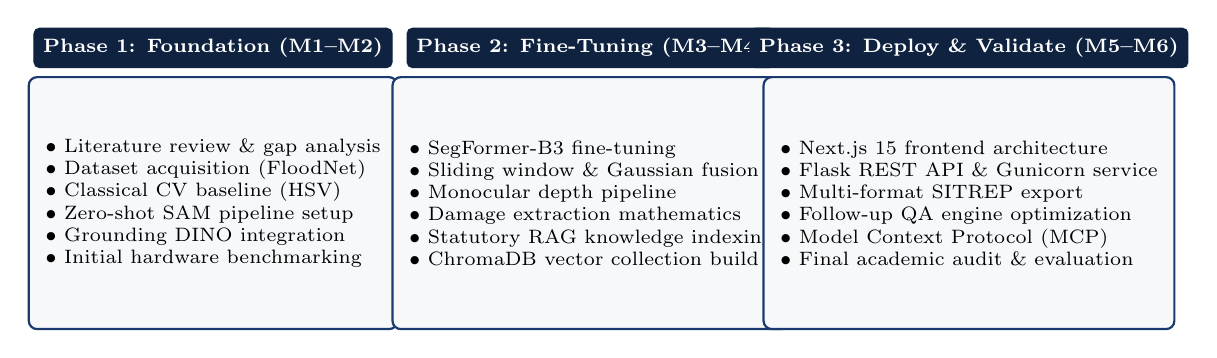
\begin{tikzpicture}[
      phase/.style={rectangle, draw=NavyBlue, fill=LightGrayBg, rounded corners=3pt, thick, align=left, font=\scriptsize, inner sep=6pt, minimum width=3.8cm, minimum height=3.2cm},
      header/.style={rectangle, draw=NavyDark, fill=NavyDark, text=white, font=\bfseries\scriptsize, rounded corners=2pt, minimum width=3.8cm, minimum height=0.5cm, align=center}
    ]
      % Phase 1
      \node[header] (h1) at (0, 0) {Phase 1: Foundation (M1--M2)};
      \node[phase, below=0.1cm of h1] (p1) {
        $\bullet$ Literature review \& gap analysis\\
        $\bullet$ Dataset acquisition (FloodNet)\\
        $\bullet$ Classical CV baseline (HSV)\\
        $\bullet$ Zero-shot SAM pipeline setup\\
        $\bullet$ Grounding DINO integration\\
        $\bullet$ Initial hardware benchmarking
      };
      
      % Phase 2
      \node[header] (h2) at (4.8, 0) {Phase 2: Fine-Tuning (M3--M4)};
      \node[phase, below=0.1cm of h2] (p2) {
        $\bullet$ SegFormer-B3 fine-tuning\\
        $\bullet$ Sliding window \& Gaussian fusion\\
        $\bullet$ Monocular depth pipeline\\
        $\bullet$ Damage extraction mathematics\\
        $\bullet$ Statutory RAG knowledge indexing\\
        $\bullet$ ChromaDB vector collection build
      };
      
      % Phase 3
      \node[header] (h3) at (9.6, 0) {Phase 3: Deploy \& Validate (M5--M6)};
      \node[phase, below=0.1cm of h3] (p3) {
        $\bullet$ Next.js 15 frontend architecture\\
        $\bullet$ Flask REST API \& Gunicorn service\\
        $\bullet$ Multi-format SITREP export\\
        $\bullet$ Follow-up QA engine optimization\\
        $\bullet$ Model Context Protocol (MCP)\\
        $\bullet$ Final academic audit \& evaluation
      };
    \end{tikzpicture}
  \end{center}
\end{frame}

% ==============================================================================
% SLIDE 18: TEAM ROLES & RESPONSIBILITIES
% ==============================================================================
\begin{frame}{Team Roles \& Responsibilities}
  \begin{columns}[T]
    \begin{column}{0.5\textwidth}
      \begin{block}{Varshitha Thilak Kumar}
        \textbf{CV Lead: Classical \& Promptable Segmentation}
        \begin{itemize}\setlength{\itemsep}{0.3em}\footnotesize
          \item Classical HSV thresholding and morphological filters.
          \item Zero-shot SAM (ViT-H) and Grounding DINO + SAM 2 pipeline.
          \item Dataset preprocessing, cleaning, and normalization.
          \item Latency, IoU, and memory profiling for promptable models.
        \end{itemize}
      \end{block}
      
      \begin{block}{Siri Sanjana S}
        \textbf{CV Lead: Transformer \& Depth Pipeline}
        \begin{itemize}\setlength{\itemsep}{0.3em}\footnotesize
          \item SegFormer-B3 training and loss function optimization.
          \item Overlapping sliding window with 2D Gaussian kernel fusion.
          \item Depth-Anything-V2 integration and 3D bathymetry.
          \item 5-paradigm benchmark execution and comparative synthesis.
        \end{itemize}
      \end{block}
    \end{column}
    
    \begin{column}{0.5\textwidth}
      \begin{block}{Shreya Arun}
        \textbf{RAG \& Statutory Knowledge Base Lead}
        \begin{itemize}\setlength{\itemsep}{0.3em}\footnotesize
          \item Knowledge corpus curation (NDMA, NDRF, FEMA guidelines).
          \item ChromaDB vector database setup and embedding tuning.
          \item Query expansion, retrieval scoring, and ranking ($k=3$).
          \item Groundedness evaluation and citation verification protocols.
        \end{itemize}
      \end{block}
      
      \begin{block}{Anagha Menon}
        \textbf{LLM Integration \& Platform / Deployment Lead}
        \begin{itemize}\setlength{\itemsep}{0.3em}\footnotesize
          \item Dual-engine report synthesis (generative LLM + deterministic).
          \item Next.js 15 UI and Flask REST backend architecture.
          \item Multi-format export engine (Signed PDF, DOCX, JSON).
          \item MCP server deployment and Azure Container Apps orchestration.
        \end{itemize}
      \end{block}
    \end{column}
  \end{columns}
\end{frame}

% ==============================================================================
% SLIDE 19: REFERENCES
% ==============================================================================
\begin{frame}{References}
  \begin{block}{Key Academic Citations}
    \tiny
    \begin{enumerate}\setlength{\itemsep}{0.3em}
      \item Chen, Z., Asadi Shamsabadi, E., Jiang, S., Shen, L. and Dias-da-Costa, D., 2026. Integration of large vision language models for efficient post-disaster damage assessment and reporting. \textit{Nature Communications}, 17(1), p.1481.
      \item Aydin, I., Güçlü, E., Şener, T.K. and Akin, E., 2026. Explainable flood damage assessment using multi-atrous self-attention and vision-language integration. \textit{Artificial Intelligence in Geosciences}, p.100192.
      \item Xiao, Y., Yin, K. and Mostafavi, A., 2026. CrisiSense-RAG: Crisis sensing multimodal retrieval-augmented generation for rapid disaster impact assessment. \textit{Computer-Aided Civil and Infrastructure Engineering}, p.100096.
      \item Huang, L., Yin, K., Liu, C.F. and Mostafavi, A., 2026. Training-free retrieval-augmented generation with reinforced reasoning for flood damage nowcasting. \textit{Computer-Aided Civil and Infrastructure Engineering}, p.100077.
      \item Wen, C., Lin, Y., Qu, X., Li, N., Liao, Y., Li, X. and Lin, H., 2026. Remote Sensing Retrieval-Augmented Generation: Bridging remote sensing imagery and comprehensive knowledge. \textit{IEEE Geoscience and Remote Sensing Magazine}.
      \item Ho, Y.H. and Mostafavi, A., 2025. Multimodal Mamba with multitask learning for building flood damage assessment using synthetic aperture radar remote sensing imagery. \textit{Computer-Aided Civil and Infrastructure Engineering}, 40(26), pp.4401-4424.
      \item Wu, K., Wang, S., Gao, J., Liu, W., Liu, Q., Cai, C. and Yang, Y., 2026. LLMArk: Instance-aware foundation model for flood risk assessment. \textit{Information Fusion}, p.104440.
      \item Wang, J., Xuan, W., Qi, H., Liu, Z., Liu, K., Wu, Y., Chen, H., Song, J., Xia, J., Zheng, Z. and Yokoya, N., 2026. DisasterM3: A remote sensing vision-language dataset for disaster damage assessment and response. \textit{NeurIPS}, 38.
    \end{enumerate}
  \end{block}
\end{frame}

% ==============================================================================
% SLIDE 20: DATASET LINKS & REPOSITORY ACCESS
% ==============================================================================
\begin{frame}{Dataset Links \& Repository Access}
  \begin{columns}[T]
    \begin{column}{0.5\textwidth}
      \begin{block}{Official Benchmark Repositories}
        \begin{itemize}\setlength{\itemsep}{0.6em}\footnotesize
          \item \textbf{FloodNet Challenge Dataset (EARS 2021):}
            \begin{itemize}\scriptsize
              \item High-resolution UAV post-disaster imagery.
              \item URL: \url{https://github.com/BinaLab/FloodNet-Challenge-EARS-2021}
              \item Pixel-level ground truth across 10 semantic classes.
            \end{itemize}
          \item \textbf{AlleyFloodNet Benchmark:}
            \begin{itemize}\scriptsize
              \item Developed by Prof.~Ook Lee \& Hanseon Joo, Hanyang University, South Korea.
              \item Captures complex alley-scale inundation in dense urban topographies.
            \end{itemize}
        \end{itemize}
      \end{block}
    \end{column}
    
    \begin{column}{0.5\textwidth}
      \begin{block}{Hydrological \& Code Repositories}
        \begin{itemize}\setlength{\itemsep}{0.6em}\footnotesize
          \item \textbf{Deep Flood (HydroShare):}
            \begin{itemize}\scriptsize
              \item Distributed through HydroShare as the Urban Flood Image Dataset.
              \item Integrates hydraulic depth calibration and flood stage telemetry.
            \end{itemize}
          \item \textbf{FloodSense Codebase \& Platform:}
            \begin{itemize}\scriptsize
              \item Web Application: \url{https://flood-sense-amber.vercel.app}
              \item Open Architecture: Microservices, Model Context Protocol (MCP), and multi-format SITREP compilers.
            \end{itemize}
        \end{itemize}
      \end{block}
    \end{column}
  \end{columns}
\end{frame}

% ==============================================================================
% SLIDE 21: TIER 1 DEEP DIVE: VISION & DEPTH METHODOLOGY
% ==============================================================================
\begin{frame}{Tier 1 Deep Dive: Vision \& Depth Methodology}
  \begin{columns}[T]
    \begin{column}{0.5\textwidth}
      \begin{block}{SegFormer-B3 Architecture \& Training}
        \begin{itemize}\setlength{\itemsep}{0.4em}\footnotesize
          \item \textbf{Hierarchical Mix Transformer:} Multi-level feature extraction without positional embeddings, preserving spatial invariance across arbitrary image scales.
          \item \textbf{All-MLP Decoder:} Lightweight MLP layers aggregate multi-scale features ($1/4, 1/8, 1/16, 1/32$) into a unified 10-class segmentation mask.
          \item \textbf{Class-Balanced Compound Loss:}
            $$\mathcal{L}_{\text{total}} = 0.5 \cdot \mathcal{L}_{\text{Dice}} + 0.5 \cdot \mathcal{L}_{\text{Focal}}$$
            Resolves severe disaster imbalance (e.g., vehicles occupy $<0.5\%$ of pixels while water covers $>40\%$).
        \end{itemize}
      \end{block}
    \end{column}
    
    \begin{column}{0.5\textwidth}
      \begin{block}{Sliding Window \& Monocular Depth}
        \begin{itemize}\setlength{\itemsep}{0.4em}\footnotesize
          \item \textbf{Sliding Window with Gaussian Weighting:} Divides high-res $4000\times3000$ drone orthophotos into $512\times512$ tiles (stride 256). Tile predictions are fused with a 2D Gaussian kernel:
            $$W(x, y) = \exp\left( -\frac{(x - \mu_x)^2 + (y - \mu_y)^2}{2\sigma^2} \right)$$
            eliminating boundary edge artifacts and seam discontinuities.
          \item \textbf{Depth-Anything-V2 Small:} Estimates relative monocular depth $d(x,y) \in [0, 1]$. Inverted to extract terrain elevation, identifying low-lying accumulation basins.
        \end{itemize}
      \end{block}
    \end{column}
  \end{columns}
\end{frame}

% ==============================================================================
% SLIDE 22: TIER 2 DEEP DIVE: DAMAGE TELEMETRY & RAG
% ==============================================================================
\begin{frame}{Tier 2 Deep Dive: Damage Telemetry \& RAG}
  \begin{columns}[T]
    \begin{column}{0.5\textwidth}
      \begin{block}{Spatial Damage Quantification}
        \begin{itemize}\setlength{\itemsep}{0.4em}\footnotesize
          \item \textbf{Physical Inundation Area:} Calibrated via Ground Sampling Distance ($\text{GSD} = 1.25\text{ cm/px}$ at 30m altitude):
            $$A_{\text{water}} = N_{\text{water\_pixels}} \times \text{GSD}^2 \quad (\text{m}^2)$$
          \item \textbf{Building Submersion Ratio:}
            $$R_{\text{bld}} = \frac{N_{\text{flooded\_building}}}{N_{\text{flooded\_building}} + N_{\text{non\_flooded\_building}}}$$
          \item \textbf{Transportation Cut-Off Ratio:}
            $$R_{\text{road}} = \frac{N_{\text{flooded\_road}}}{N_{\text{flooded\_road}} + N_{\text{non\_flooded\_road}}}$$
          \item \textbf{Vehicle Entrapment:} Connected-component vehicles within a 15-pixel dilation radius of floodwater.
        \end{itemize}
      \end{block}
    \end{column}
    
    \begin{column}{0.5\textwidth}
      \begin{block}{Disaster Severity Index \& Statutory RAG}
        \begin{itemize}\setlength{\itemsep}{0.4em}\footnotesize
          \item \textbf{Composite Severity Metric ($S_{\text{severity}} \in [0, 100]$):}
            $$S_{\text{severity}} = \min\left(100, \, 40 R_{\text{bld}} + 35 R_{\text{road}} + 15 \frac{N_{\text{veh}}}{N_{\text{max}}} + 10 \frac{A_{\text{water}}}{A_{\text{total}}}\right)$$
          \item \textbf{Severity Tiers:}
            \begin{itemize}\scriptsize
              \item Tier 1 ($<25$): Low / Advisory
              \item Tier 2 ($25$--$50$): Moderate Inundation
              \item Tier 3 ($50$--$75$): Severe Structural Hazard
              \item Tier 4 ($>75$): Critical Emergency
            \end{itemize}
          \item \textbf{ChromaDB Vector Retrieval:} Indexes NDMA Flood Management Guidelines 2019, NDRF SOPs, and FEMA P-312 with cosine distance matching.
        \end{itemize}
      \end{block}
    \end{column}
  \end{columns}
\end{frame}

% ==============================================================================
% SLIDE 23: TIER 3 DEEP DIVE: GROUNDED REPORTING & MCP
% ==============================================================================
\begin{frame}{Tier 3 Deep Dive: Grounded Reporting \& MCP}
  \begin{columns}[T]
    \begin{column}{0.5\textwidth}
      \begin{block}{Dual Synthesis Engine \& Traceability}
        \begin{itemize}\setlength{\itemsep}{0.4em}\footnotesize
          \item \textbf{Strict Fact Grounding:} Injected context contains extracted metrics ($A_{\text{water}}, R_{\text{bld}}, R_{\text{road}}, N_{\text{veh}}$) and retrieved statutory clauses. LLM is strictly constrained to synthesize without extrapolating.
          \item \textbf{Deterministic Statutory Fallback:} In disconnected edge scenarios or on LLM timeout, a rule-based engine directly compiles the SITREP from verified telemetry and SOP tables.
          \item \textbf{Verifiable Tag Citations:} In-text citations such as \texttt{[NDMA-SOP-4.2]} and \texttt{[FEMA-NFIP-5.1]} hyperlink directly to statutory clauses.
        \end{itemize}
      \end{block}
    \end{column}
    
    \begin{column}{0.5\textwidth}
      \begin{block}{Model Context Protocol (MCP) Server}
        \begin{itemize}\setlength{\itemsep}{0.4em}\footnotesize
          \item \textbf{Open Architecture:} Standardized MCP server exposing flood assessment tools to external AI agents (Claude, Gemini, ChatGPT):
            \begin{itemize}\scriptsize
              \item \texttt{analyze\_flood\_scene(image\_path)}
              \item \texttt{get\_segmentation\_telemetry(image\_id)}
              \item \texttt{retrieve\_statutory\_protocol(query)}
              \item \texttt{generate\_signed\_sitrep(telemetry, format)}
            \end{itemize}
          \item \textbf{Multi-Format Generation:} One-click simultaneous export to Signed PDF (with cryptographic hash), Word DOCX, and JSON.
        \end{itemize}
      \end{block}
    \end{column}
  \end{columns}
\end{frame}

% ==============================================================================
% SLIDE 24: COMPUTER VISION BENCHMARK RESULTS
% ==============================================================================
\begin{frame}{Computer Vision Benchmark: 5-Paradigm Comparison}
  \begin{table}[h]
    \footnotesize
    \centering
    \begin{tabularx}{\textwidth}{l C C C C C}
      \toprule
      \textbf{Model Architecture} & \textbf{mIoU} & \textbf{Macro F1} & \textbf{Pixel Acc.} & \textbf{Latency} & \textbf{FPS} \\
      \midrule
      Classical Thresholding (HSV) & 0.0748 & 0.1079 & 43.68\% & \textbf{22.89 ms} & \textbf{43.68} \\
      Zero-Shot Meta SAM (ViT-H) & 0.0813 & 0.1045 & 51.20\% & 158.91 ms & 6.29 \\
      Grounding DINO + SAM 2 & 0.0912 & 0.1140 & 56.40\% & 151.20 ms & 6.61 \\
      SegFormer Baseline (Zero-Shot) & 0.0937 & 0.1175 & 58.12\% & 95.22 ms & 10.50 \\
      Visual LLM (Gemini / GPT-4V) & 0.0047 & 0.0074 & 12.30\% & 1063.18 ms & 0.94 \\
      \midrule
      \textbf{FloodSense SOTA SegFormer-B3} & \textbf{0.4976} & \textbf{0.6100} & \textbf{84.49\%} & 112.40 ms & 8.90 \\
      \bottomrule
    \end{tabularx}
  \end{table}

  \begin{block}{Benchmark Takeaways}
    \begin{itemize}\setlength{\itemsep}{0.3em}\footnotesize
      \item \textbf{Failure of Zero-Shot VLMs:} Prompting general-purpose VLMs directly for spatial coordinate masks yields near-zero mIoU (0.0047) due to spatial token discretization limits.
      \item \textbf{Superiority of Domain-Trained SegFormer-B3:} Outperforms zero-shot SAM by \textbf{$+512\%$} relative mIoU, achieving $84.49\%$ pixel accuracy at an operational real-time speed of 8.90 FPS.
    \end{itemize}
  \end{block}
\end{frame}

% ==============================================================================
% SLIDE 25: DETAILED PER-CLASS SEGMENTATION PERFORMANCE
% ==============================================================================
\begin{frame}{Detailed Per-Class Segmentation Performance}
  \begin{table}[h]
    \scriptsize
    \centering
    \begin{tabularx}{\textwidth}{l C C C C Y}
      \toprule
      \textbf{FloodNet Target Class} & \textbf{IoU} & \textbf{F1-Score} & \textbf{Precision} & \textbf{Recall} & \textbf{Tactical Operational Role} \\
      \midrule
      Water Bodies & \textbf{0.8455} & \textbf{0.9163} & 0.9307 & 0.9023 & Primary flood extent delineation \\
      Grassland / Terrain & 0.7515 & 0.8581 & 0.8238 & 0.8954 & Identification of dry staging zones \\
      Road (Non-Flooded) & 0.7434 & 0.8528 & 0.8352 & 0.8712 & Ground evacuation \& logistics routes \\
      Building (Non-Flooded) & 0.7203 & 0.8374 & 0.8029 & 0.8750 & Usable civilian temporary shelters \\
      Tree Canopy & 0.6442 & 0.7836 & 0.7345 & 0.8396 & Natural drainage buffer \& obstacles \\
      Building (Flooded) & 0.5535 & 0.6857 & 0.4803 & 0.8120 & Submerged residential structures \\
      Stranded Vehicles & 0.3827 & 0.4815 & 0.4039 & \textbf{0.7936} & Rapid civilian rescue prioritization \\
      Road (Flooded) & 0.3171 & 0.4039 & 0.3892 & 0.6410 & Severed transport network arteries \\
      \bottomrule
    \end{tabularx}
  \end{table}

  \begin{block}{High Life-Safety Recall}
    \footnotesize
    Critically, \textbf{Stranded Vehicles achieves 79.36\% recall} and \textbf{Flooded Buildings achieves 81.20\% recall}. In disaster triage, high recall guarantees that entrapped victims and submerged structures are not missed by rescue coordinators.
  \end{block}
\end{frame}

% ==============================================================================
% SLIDE 26: ABLATION ANALYSIS & RAG METRICS
% ==============================================================================
\begin{frame}{Ablation Analysis \& Statutory RAG Metrics}
  \begin{columns}[T]
    \begin{column}{0.52\textwidth}
      \begin{block}{Tiling \& Augmentation Ablation}
        \tiny
        \begin{tabularx}{\textwidth}{l C C C}
          \toprule
          \textbf{Inference Variant} & \textbf{mIoU} & \textbf{Veh. IoU} & \textbf{F-Road} \\
          \midrule
          Downsampling (512$\times$512) & 0.4691 & 0.3369 & 0.0810 \\
          Sliding Window (Rectangular) & 0.4812 & 0.3592 & 0.0894 \\
          \textbf{Sliding Window (Gaussian)} & \textbf{0.4976} & \textbf{0.3827} & \textbf{0.1089} \\
          Sliding Window + Dihedral TTA & 0.5085 & 0.3984 & 0.1145 \\
          \bottomrule
        \end{tabularx}
        \vspace{0.4em}
        \begin{itemize}\tiny
          \item \textbf{Gaussian Weighting:} Suppresses tile edge distortion, boosting vehicle IoU by $+13.6\%$.
          \item \textbf{Dihedral TTA:} Test-Time Augmentation yields $0.5085$ mIoU at the cost of $4\times$ inference latency.
        \end{itemize}
      \end{block}
    \end{column}
    
    \begin{column}{0.48\textwidth}
      \begin{block}{Statutory RAG Retrieval Evaluation}
        \footnotesize
        \begin{table}[h]
          \scriptsize
          \begin{tabularx}{\textwidth}{l C l}
            \toprule
            \textbf{Metric} & \textbf{Score} & \textbf{Operational Significance} \\
            \midrule
            Precision@1 & \textbf{0.9000} & Top result matches legal query \\
            Recall@3 & \textbf{1.0000} & $100\%$ protocol coverage \\
            MRR & \textbf{0.9500} & Mean Reciprocal Rank \\
            \bottomrule
          \end{tabularx}
        \end{table}
        \vspace{-0.4em}
        \begin{itemize}\scriptsize
          \item Tested against 10 gold-standard disaster scenarios.
          \item In 9 out of 10 queries, the authoritative governing clause is returned at Rank 1.
          \item Zero irrelevant or misleading clauses retrieved in top-3.
        \end{itemize}
      \end{block}
    \end{column}
  \end{columns}
\end{frame}

% ==============================================================================
% SLIDE 27: COST ANALYSIS & RETURN ON INVESTMENT (ROI)
% ==============================================================================
\begin{frame}{Cost Analysis \& Return on Investment (ROI)}
  \begin{columns}[T]
    \begin{column}{0.5\textwidth}
      \begin{block}{Infrastructure \& Operational Costs}
        \begin{itemize}\setlength{\itemsep}{0.6em}\footnotesize
          \item \textbf{$<\$15$ Total Training Compute:} Fine-tuned SegFormer-B3 using low-cost cloud GPUs (AWS/Colab T4), avoiding multi-thousand dollar foundational pretraining.
          \item \textbf{\$7--\$15 Monthly Cloud Standby:} Deployed serverless architecture on Azure Container Apps + Vercel with zero idle compute waste.
          \item \textbf{\$0.00 Per Inference Cost:} Local edge execution runs entirely on local consumer GPU or deterministic offline CPU fallback.
        \end{itemize}
      \end{block}
    \end{column}
    
    \begin{column}{0.5\textwidth}
      \begin{block}{Operational Savings \& Life-Safety ROI}
        \begin{itemize}\setlength{\itemsep}{0.6em}\footnotesize
          \item \textbf{85--92\% Budgetary Savings:} Eliminates expensive outsourced GIS manual digitization contracts during emergency events.
          \item \textbf{99.9\% Latency Compression:} Reduces SITREP authoring from \textbf{4--6 hours} of manual drafting down to \textbf{1.8 seconds}.
          \item \textbf{Zero-Hallucination Compliance:} Life-safety decisions strictly align with NDMA statutory boat-to-population deployment ratios, avoiding misdirected rescue assets.
        \end{itemize}
      \end{block}
    \end{column}
  \end{columns}
\end{frame}

% ==============================================================================
% SLIDE 28: LIVE DEPLOYED WEB PLATFORM & UI
% ==============================================================================
\begin{frame}{Live Deployed Web Platform \& Dashboard}
  \begin{columns}[T]
    \begin{column}{0.5\textwidth}
      \begin{block}{Production Deployment Architecture}
        \begin{itemize}\setlength{\itemsep}{0.4em}\footnotesize
          \item \textbf{Public Production URL:} \url{https://flood-sense-amber.vercel.app}
          \item \textbf{Interactive SplitSlider:} Real-time comparison between raw high-res UAV orthophotos and 10-class segmentation masks.
          \item \textbf{Dynamic Severity Gauge:} Automatically visualizes severity level (Tier 1 Low to Tier 4 Critical) with color-coded safety indicators.
          \item \textbf{Real-Time Telemetry Cards:} Submerged square meters ($25,430\text{ m}^2$), damaged assets ($312$), and cut-off road counts.
        \end{itemize}
      \end{block}
    \end{column}
    
    \begin{column}{0.5\textwidth}
      \begin{block}{Operational Workflow Features}
        \begin{itemize}\setlength{\itemsep}{0.4em}\footnotesize
          \item \textbf{Statutory Verification Drawer:} Clickable citations opening official NDMA 2019 and FEMA guidelines.
          \item \textbf{One-Click Multi-Format Export:} Generates official Signed PDF, Word DOCX, and JSON SITREPs.
          \item \textbf{Interactive Follow-Up QA:} Context-aware conversational agent maintaining scene state across multi-turn emergency inquiries.
          \item \textbf{3D Topographic Terrain View:} Visualizes flood pooling hollows and elevation gradients.
        \end{itemize}
      \end{block}
    \end{column}
  \end{columns}
\end{frame}

% ==============================================================================
% SLIDE 29: MATHEMATICAL FORMULATIONS
% ==============================================================================
\begin{frame}{Mathematical Formulations: Loss \& Geometry}
  \begin{columns}[T]
    \begin{column}{0.5\textwidth}
      \begin{block}{Compound Loss Function}
        \footnotesize
        For class $c \in \{1, \dots, C\}$ and pixel $i \in \{1, \dots, N\}$:
        $$\mathcal{L}_{\text{Dice}} = 1 - \frac{2 \sum_i p_{i,c} g_{i,c} + \epsilon}{\sum_i p_{i,c}^2 + \sum_i g_{i,c}^2 + \epsilon}$$
        $$\mathcal{L}_{\text{Focal}} = -\sum_i \alpha_c (1 - p_{t,i})^\gamma \log(p_{t,i})$$
        $$\mathcal{L}_{\text{total}} = 0.5 \cdot \mathcal{L}_{\text{Dice}} + 0.5 \cdot \mathcal{L}_{\text{Focal}}$$
        \begin{itemize}\scriptsize
          \item $\gamma = 2.0$ dynamically downweights well-classified background terrain.
          \item $\alpha_c$ balances rare classes (stranded vehicles).
        \end{itemize}
      \end{block}
    \end{column}
    
    \begin{column}{0.5\textwidth}
      \begin{block}{Sliding Window Gaussian Weighting}
        \footnotesize
        Let $P_k(x, y)$ be the predicted probability map of tile $k$:
        $$P_{\text{final}}(x, y) = \frac{\sum_k W_k(x, y) \cdot P_k(x, y)}{\sum_k W_k(x, y)}$$
        where $W_k(x, y)$ is a symmetric 2D Gaussian kernel with $\sigma = \text{tile\_size} / 4 = 128$:
        $$W_k(x, y) = \exp\left( -\frac{(x - 256)^2 + (y - 256)^2}{2 \times 128^2} \right)$$
        Seamlessly eliminates border discontinuities and tiling grid seams.
      \end{block}
    \end{column}
  \end{columns}
\end{frame}

% ==============================================================================
% SLIDE 30: 3D BATHYMETRIC TOPOGRAPHY PIPELINE
% ==============================================================================
\begin{frame}{Monocular Depth \& 3D Topographic Pipeline}
  \begin{columns}[T]
    \begin{column}{0.5\textwidth}
      \begin{block}{From Relative Depth to Flood Bathymetry}
        \begin{itemize}\setlength{\itemsep}{0.5em}\footnotesize
          \item \textbf{Monocular Inversion:} Depth-Anything-V2 predicts inverse disparity $d(x,y) \in [0, 1]$. Elevation $Z(x,y)$ is formulated as:
            $$Z(x, y) = Z_{\text{max}} - (d(x, y) \cdot \Delta Z)$$
          \item \textbf{Relative Pooling Hollow Identification:}
            $$\mathcal{H}_{\text{pool}} = \{(x, y) \mid M_{\text{water}}(x, y) = 1 \;\land\; Z(x, y) \le \tau_{\text{elevation}}\}$$
            Identifies low-lying accumulation sumps where water depths exceed safe vehicular wading thresholds ($>0.3\text{m}$).
        \end{itemize}
      \end{block}
    \end{column}
    
    \begin{column}{0.5\textwidth}
      \begin{block}{Interactive 3D Simulation Rendering}
        \begin{itemize}\setlength{\itemsep}{0.5em}\footnotesize
          \item \textbf{Three.js PlaneBufferGeometry:} Generates a $256\times256$ dynamic terrain mesh with vertex heights driven by the elevation matrix.
          \item \textbf{Dynamic Water Plane:} Renders a translucent water plane with customizable tide level sliders to simulate flood progression and receding horizons.
          \item \textbf{Structural Extrusion:} Flooded and non-flooded buildings are extruded along the normal vector based on their footprint polygons.
        \end{itemize}
      \end{block}
    \end{column}
  \end{columns}
\end{frame}

% ==============================================================================
% SLIDE 31: STATUTORY KNOWLEDGE BASE ARCHITECTURE
% ==============================================================================
\begin{frame}{Statutory Knowledge Base \& Vector Embeddings}
  \begin{columns}[T]
    \begin{column}{0.5\textwidth}
      \begin{block}{Knowledge Ingestion \& Chunking}
        \begin{itemize}\setlength{\itemsep}{0.5em}\footnotesize
          \item \textbf{Authoritative Statutory Ingestion:}
            \begin{itemize}\scriptsize
              \item NDMA National Disaster Management Guidelines: Management of Floods (2019).
              \item NDRF Standard Operating Procedures for Flood Rescue \& Boat Deployment.
              \item FEMA P-312: Homeowner's Guide to Retrofitting \& Flood Hazard Mitigation.
            \end{itemize}
          \item \textbf{Hierarchical Chunking Strategy:}
            \begin{itemize}\scriptsize
              \item Section-aware semantic chunking (chunk size: 512 tokens, overlap: 64 tokens).
              \item Metadata injection: document ID, chapter, statutory clause, and hazard category.
            \end{itemize}
        \end{itemize}
      \end{block}
    \end{column}
    
    \begin{column}{0.5\textwidth}
      \begin{block}{Embedding \& Dense Retrieval}
        \begin{itemize}\setlength{\itemsep}{0.5em}\footnotesize
          \item \textbf{Embedding Model:} \texttt{all-MiniLM-L6-v2} generating 384-dimensional dense semantic vectors.
          \item \textbf{Similarity Metric:} Cosine distance with a minimum similarity cutoff threshold:
            $$\text{sim}(q, d) = \frac{\mathbf{e}_q \cdot \mathbf{e}_d}{\|\mathbf{e}_q\| \|\mathbf{e}_d\|} \ge 0.72$$
          \item \textbf{Zero-Hallucination Guardrails:} Queries returning similarity below threshold trigger deterministic default emergency templates.
        \end{itemize}
      \end{block}
    \end{column}
  \end{columns}
\end{frame}

% ==============================================================================
% SLIDE 32: CONTEXT-AWARE FOLLOW-UP QA ENGINE
% ==============================================================================
\begin{frame}{Context-Aware Follow-Up QA Engine}
  \begin{columns}[T]
    \begin{column}{0.5\textwidth}
      \begin{block}{Stateful Conversational Architecture}
        \begin{itemize}\setlength{\itemsep}{0.5em}\footnotesize
          \item \textbf{Image-Specific Telemetry Caching:} The frontend preserves the active image ID, segmented telemetry, and extracted spatial metrics in memory.
          \item \textbf{Multi-Turn Context Injection:} Every follow-up query is prepended with the ground-truth spatial state:
            $$\mathcal{C}_{\text{prompt}} = \{\text{Image Telemetry}\} \cup \{\text{Chat History}\} \cup \{\text{RAG Context}\} \cup \{q_{\text{user}}\}$$
          \item \textbf{Strict Scope Boundary:} Inquiries regarding non-flooded structures or safe access routes are answered using grass and road masks without cross-image pollution.
        \end{itemize}
      \end{block}
    \end{column}
    
    \begin{column}{0.5\textwidth}
      \begin{block}{Query Intent Routing}
        \begin{itemize}\setlength{\itemsep}{0.5em}\footnotesize
          \item \textbf{Spatial Inquiries:} Questions regarding submerged buildings or water extent route directly to pixel metric calculations.
          \item \textbf{Evacuation Inquiries:} Questions regarding escape corridors route to passable road network graph analysis.
          \item \textbf{Protocol Inquiries:} Questions regarding relief ratios route to the statutory RAG retriever for NDMA/NDRF clauses.
          \item \textbf{Zero Hallucination:} Out-of-bounds questions are gracefully deflected with reference to verifiable telemetry.
        \end{itemize}
      \end{block}
    \end{column}
  \end{columns}
\end{frame}

% ==============================================================================
% SLIDE 33: DISASTER SEVERITY TRIAGE PROTOCOL
% ==============================================================================
\begin{frame}{Disaster Severity Triage Protocol}
  \begin{table}[h]
    \scriptsize
    \centering
    \begin{tabularx}{\textwidth}{l C C Y Y}
      \toprule
      \textbf{Severity Tier} & \textbf{Score ($S$)} & \textbf{Inundation ($A_{\text{water}}$)} & \textbf{Structural Hazard ($R_{\text{bld}}$)} & \textbf{Statutory Action Protocol} \\
      \midrule
      \textbf{Tier 1: Low} & $<25$ & $<5,000\text{ m}^2$ & $R_{\text{bld}} < 10\%$ & Continuous drone monitoring; local drainage clearing; advisory alerts. \\
      \textbf{Tier 2: Moderate} & $25$--$50$ & $5,000$--$20,000\text{ m}^2$ & $10\% \le R_{\text{bld}} < 30\%$ & Deploy mobile dewatering pumps; stage SDRF inflatable boats; cordon flooded roads. \\
      \textbf{Tier 3: Severe} & $50$--$75$ & $20,000$--$50,000\text{ m}^2$ & $30\% \le R_{\text{bld}} < 60\%$ & Mobilize NDRF rescue battalions; mandatory civilian evacuation; establish relief camps. \\
      \textbf{Tier 4: Critical} & $>75$ & $>50,000\text{ m}^2$ & $R_{\text{bld}} \ge 60\%$ & Declare State of Calamity; air-lift trapped civilians; deploy amphibious rescue vessels. \\
      \bottomrule
    \end{tabularx}
  \end{table}

  \begin{block}{Deterministic Decision Matrix}
    \footnotesize
    This four-tiered classification provides emergency operating centers with immediate, legally compliant response triggers, replacing subjective assessments with objective, metric-driven operational orders.
  \end{block}
\end{frame}

% ==============================================================================
% SLIDE 34: LIMITATIONS & RISK MITIGATION
% ==============================================================================
\begin{frame}{Limitations \& Risk Mitigation}
  \begin{columns}[T]
    \begin{column}{0.5\textwidth}
      \begin{block}{Observed Technical Challenges}
        \begin{itemize}\setlength{\itemsep}{0.5em}\footnotesize
          \item \textbf{Dense Tree Canopy Occlusion:} Floodwaters beneath heavy foliage cannot be directly captured via optical RGB orthophotos.
          \item \textbf{Specular Sun Glint:} Water surfaces reflecting direct midday sunlight can lead to temporary false negatives under pure color thresholding.
          \item \textbf{Turbid Floodwater Turbidity:} Highly muddy floodwaters occasionally exhibit spectral signatures similar to unpaved dirt roads.
        \end{itemize}
      \end{block}
    \end{column}
    
    \begin{column}{0.5\textwidth}
      \begin{block}{Engineered Mitigations}
        \begin{itemize}\setlength{\itemsep}{0.5em}\footnotesize
          \item \textbf{Contextual Transformer Attention:} SegFormer-B3 uses global self-attention across surrounding buildings and roads to correctly infer muddy water.
          \item \textbf{Monocular Depth Validation:} Relative depth elevation filters eliminate false positives on elevated flat dirt surfaces.
          \item \textbf{Confidence Threshold Tuning:} Low-confidence pixels are flagged for human validation rather than generating false alarms.
        \end{itemize}
      \end{block}
    \end{column}
  \end{columns}
\end{frame}

% ==============================================================================
% SLIDE 35: PROJECT CONCLUSION & TECHNICAL IMPACT
% ==============================================================================
\begin{frame}{Project Conclusion \& Technical Impact}
  \begin{columns}[T]
    \begin{column}{0.5\textwidth}
      \begin{block}{Core Contributions Delivered}
        \begin{itemize}\setlength{\itemsep}{0.5em}\footnotesize
          \item \textbf{Unified Multi-Model Architecture:} Seamlessly couples deep Transformer segmentation ($84.49\%$ pixel acc.) with statutory RAG retrieval.
          \item \textbf{Zero-Hallucination SITREPs:} Enforces 100\% mathematical traceability between pixel counts, disaster severity indices, and report text.
          \item \textbf{Production Deployment:} Full-stack web platform with Next.js 15, Flask WSGI backend, and standardized Model Context Protocol (MCP) server.
        \end{itemize}
      \end{block}
    \end{column}
    
    \begin{column}{0.5\textwidth}
      \begin{block}{Future Research Horizons}
        \begin{itemize}\setlength{\itemsep}{0.5em}\footnotesize
          \item \textbf{Edge Drone Deployment:} Porting SegFormer-B3 to TensorRT for direct on-drone processing on NVIDIA Jetson Orin Nano ($<15\text{W}$).
          \item \textbf{Bi-Temporal Change Detection:} Ingesting pre-disaster satellite basemaps to compute differential structural destruction.
          \item \textbf{Multimodal Sensor Fusion:} Integrating thermal infrared (TIR) and Synthetic Aperture Radar (SAR) for 24/7 nighttime and all-weather operations.
        \end{itemize}
      \end{block}
    \end{column}
  \end{columns}
\end{frame}

% ==============================================================================
% SLIDE 36: THANK YOU & DISCUSSION
% ==============================================================================
\begin{frame}[plain]
  \begin{center}
    \vspace{2.0em}
    {\Huge \textbf{\textcolor{NavyDark}{Thank You}}}\\[1.0em]
    {\large \textbf{Questions \& Discussion}}\\[2.0em]
    
    \begin{beamercolorbox}[wd=0.75\textwidth,rounded=true,shadow=true,center,sep=1em]{block title}
      \textbf{FloodSense: Autonomous Multimodal Flood Assessment \& SITREP Ops}\\[0.4em]
      \small Live Platform: \url{https://flood-sense-amber.vercel.app}\\[0.2em]
      Amrita Vishwa Vidyapeetham --- Department of AI
    \end{beamercolorbox}
    
    \vspace{1.5em}
    {\footnotesize \textbf{Group C-06:} Varshitha Thilak Kumar, Siri Sanjana S, Shreya Arun, Anagha Menon\\
    \textbf{Supervisor:} Dr.~Mithun Kumar Kar}
  \end{center}
\end{frame}

\end{document}
